\chapter{Evaluaciones y análisis de resultados}
\label{results}

\section{Estimación del parámetro Beta}
% PRIMERO EXPLICAR COMO DEPENDE LA EJECUCION CON EL PARÁMETRO BETA
% PARA VALORES MAS CHICOS ...
% PARA VALORES MAS GRANDES...
% DAR UNA IDEA DEL RANGO DE VALORES BETA DE ACUERDO A LA ECUACION, PARA DIFERENCIAS DE SCORE = 1
% MOSTRAR GRAFICO/S DE RELACION ENTRE 
% POR LO TANTO, UN PARAMETRO QUE TIENE EN CUENTA ESTOS ASPECTOS, QUE PODRIA EVALUAR CORRECTAMENTE LA EJECUCION EN FUNCION DE BETA , Y QUE ADEMAS ES EL DATO MAS IMPORTANTE EN LA EJECUCION ES EL TIEMPO DE EJECUCION

En las secciones previas hemos propuesto un método de diseño que se basa en búsqueda estocástica sobre el espacio de secuencias.
El método de búsqueda es guiado por el resultado de una función que asigna un puntaje a cada secuencia, el cual resulta siempre mayor o igual a 0.
La secuencia resultante buscada se caracteriza por tener un puntaje igual a 0, por lo tanto, el método puede verse como la búsqueda de un mínimo global sobre la superficie
que relaciona cada posible secuencia con su valor de puntaje.

El comportamiento del método de búsqueda del diseño resultante depende de un único parámetro $\beta$ cuyo valor(o rango) óptimo está fuertemente asociado a las características de esta superficie.
% El el valor(o el rango) óptimo para el parámetro que Beta depende en gran parte de las características de esta superficie.
Un valor de $\beta$ más grande tiene un porcentaje de aceptación mayor de mutaciones que aumentan el puntaje de la secuencia, por lo tanto, permite la exploración de superficies que 
requieren superar mínimos locales para alcanzar secuencias con puntaje 0.
Un valor de beta mas chico implica recorrer un camino más directo hacia el mínimo ya que se aceptan menos mutaciones que aumenten el puntaje, pero esto podría requerir la evaluación de una gran cantidad de posibilidades. 
Incluso, si la búsqueda se estanca en un mínimo local, un valor muy chico de beta solo podría encontrar la solución en un tiempo infinitamente 
grande. Como vimos en el capítulo 2, la decisión de aceptación está basada en el uso de la ecuación \ref{monteCarlo}, la cual siempre devuelve un valor $>0$ para cualquier $\beta$ positivo.
% Para cualquier valor de $\beta$ positivo dadas las propiedades del método de decisión para aceptar las mutaciones,   el valor de la ecuación \ref{monteCarlo} siempre será mayor que 0. 
Por lo tanto, la probabilidad de aceptación nunca es 0 y no es imposible encontrar el resultado si es que existe, aún cuando el tiempo que se demore sea prácticamente infinito.

% En esta aplicación, además, partiendo de una secuencia inicial dada por el usuario, resultaría mejor obtener la secuencia con puntaje mínimo que esté más cerca en la superficie, es decir, que sea más similar a la secuencia inicial.
% Esto implica una menor cantidad de mutaciones, lo que equivale a un valor de beta mas chico.


Sin embargo, a pesar que previo a desarrollar la aplicación asumimos que el espacio de soluciones era considerablemente grande, no sabemos cómo es exactamente 
la superficie que asocia cada secuencia con el puntaje definido por las evaluaciones. 
De esta forma, inicialmente no tenemos ningún conocimiento de como se relaciona el valor del parámetro $\beta$ con la ejecución resultante.
Para tener una primera idea global de esta dependencia analizamos las ejecuciones de 6 corridas independientes.
Tres de estas corridas se realizaron a partir de secuencias generadas aleatoriamente, mientras que las tres restantes se inician a partir de secuencias naturales definidas(distintas entre si).
En todos los casos la longitud de la secuencia fue de 30 aminoácidos.
Este mismo esquema de 6 corridas se repitió para valores de $\beta=0.5$ y $\beta=2.4$.
En el caso del $\beta$ más chico(0.5), la probabilidad de aceptar una mutación para un incremento de 1 en el puntaje es de $13\%$, mientras que para el beta más grande(2.4) esta probabilidad es de $65,9\%$.
Por lo tanto, los dos valores podrían clasificarse como cercanos a los extremos dentro del esquema de decisión basado en el puntaje.
% rango de posibles valores para $\beta$.
% Los resultados de las corridas se muestran en la tabla ......... ***CONVIENE RESUMIR BIEN LOS DATOS EN UNA TABLA? EL UNICO DATO CREO QUE SERIA EL TOTAL DE ITERACIONES


% GRAFICO DE SCORE vs ITERACION   (MEDIAS Y StdDeV COMPLETO HASTA EL FINAL)   +  CORRIDAS INDIVIDUALES
En el gráfico \ref{fig:scoreVsiter} se muestra la dependencia del puntaje con las iteraciones, tanto los valores medios(y desviación estandar) para todas las ejecuciones mencionadas(gráfico \ref{fig:scoreVsiter-b}), 
como el detalle de las ejecuciones individuales(gráfico \ref{fig:scoreVsiter-a}).
El perfil que se muestra permite aclarar mejor los conceptos mencionados previamente acerca de la dependencia de $\beta$ con el comportamiento de la búsqueda. 
Un valor más grande de $\beta$ realiza una mayor exploración del espacio de soluciones, lo que se ve reflejado en un rango mucho más amplio de mutaciones aplicadas para las ejecuciones.
Se ve claramente que hay una diferencia en el orden de magnitud de la cantidad de iteraciones, donde las ejecuciones con $\beta=2.4$ pueden alcanzar $>2000$ iteraciones.
Por su parte, el valor más chico de $\beta$ permite alcanzar el objetivo en un número mucho menor de mutaciones, lo cual parece indicar que hay un camino 
que conduce desde cada punto de inicio hacia un resultado bajando continuamente el valor del puntaje, es decir, sin atravesar ninguna barrera.
De todas formas, no podemos decir nada sobre las características de este recorrido hacía el mínimo.
% PONER ALGUNA CONCLUSION DE QUE DICE ESTO ACERCA DE LA SUPERFICIE 


% 
% \begin{figure} 
% \advance\leftskip-2cm
% \subfigure[Ejecuciones individuales]{\label{fig:scoreVsiter-a}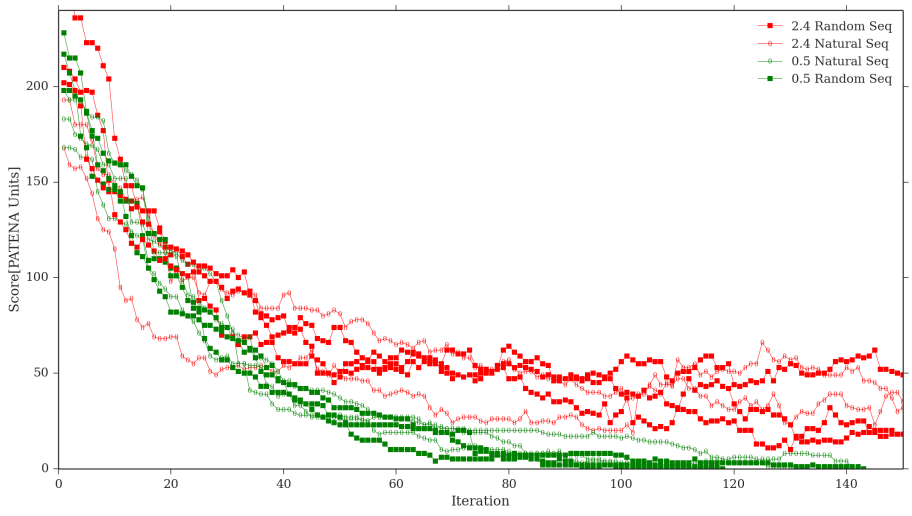
\includegraphics[width=1.15\textwidth]{img/resultados/individuales-scoreVsiter-hasta150.png}}
% \subfigure[Valores medios y desviaciones]{\label{fig:scoreVsiter-b}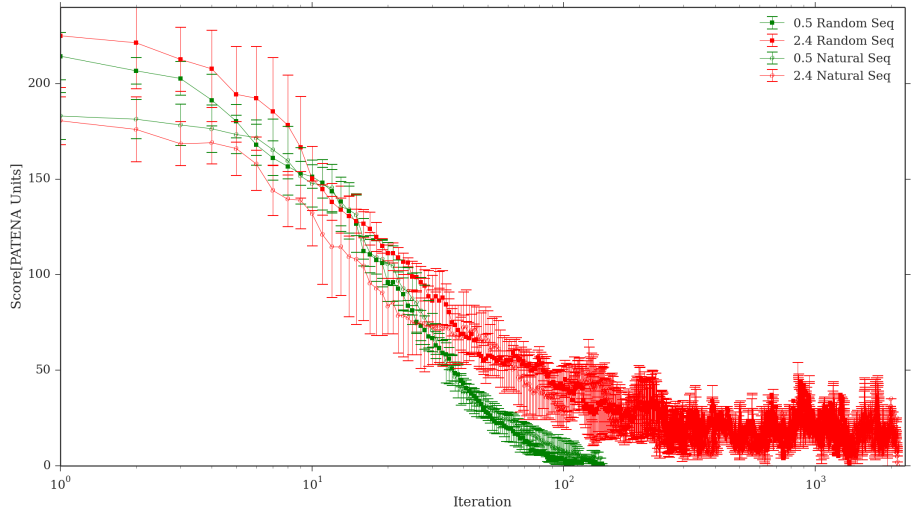
\includegraphics[width=1.15\textwidth]{img/resultados/scoreVsiter-cada1-hasta2270.png}}
%  \caption{Puntaje asociado a cada iteración}
%  \label{fig:scoreVsiter}
% 
% \end{figure}


\begin{figure}[htbp]
\advance\leftskip-1.5cm
  \begin{subfigure}[b]{\textwidth}
%     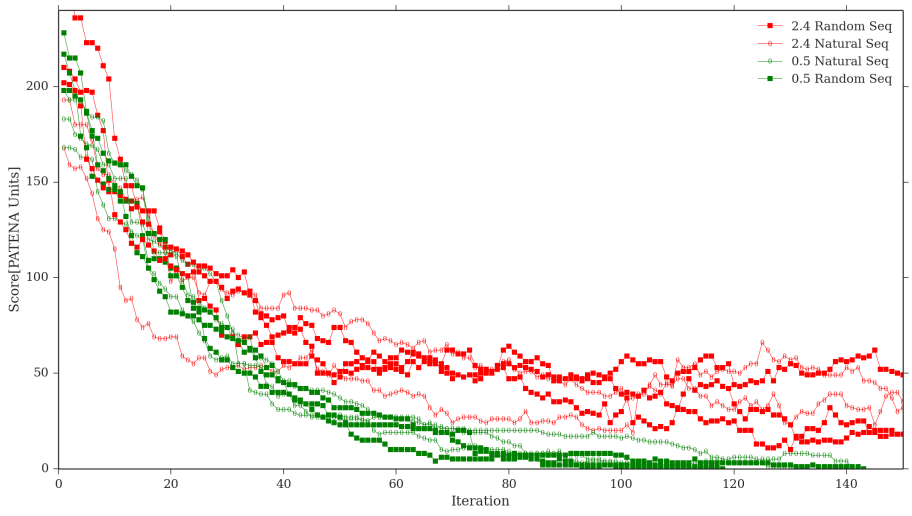
\includegraphics[width=1.15\textwidth]{img/resultados/individuales-scoreVsiter-hasta150.png}
 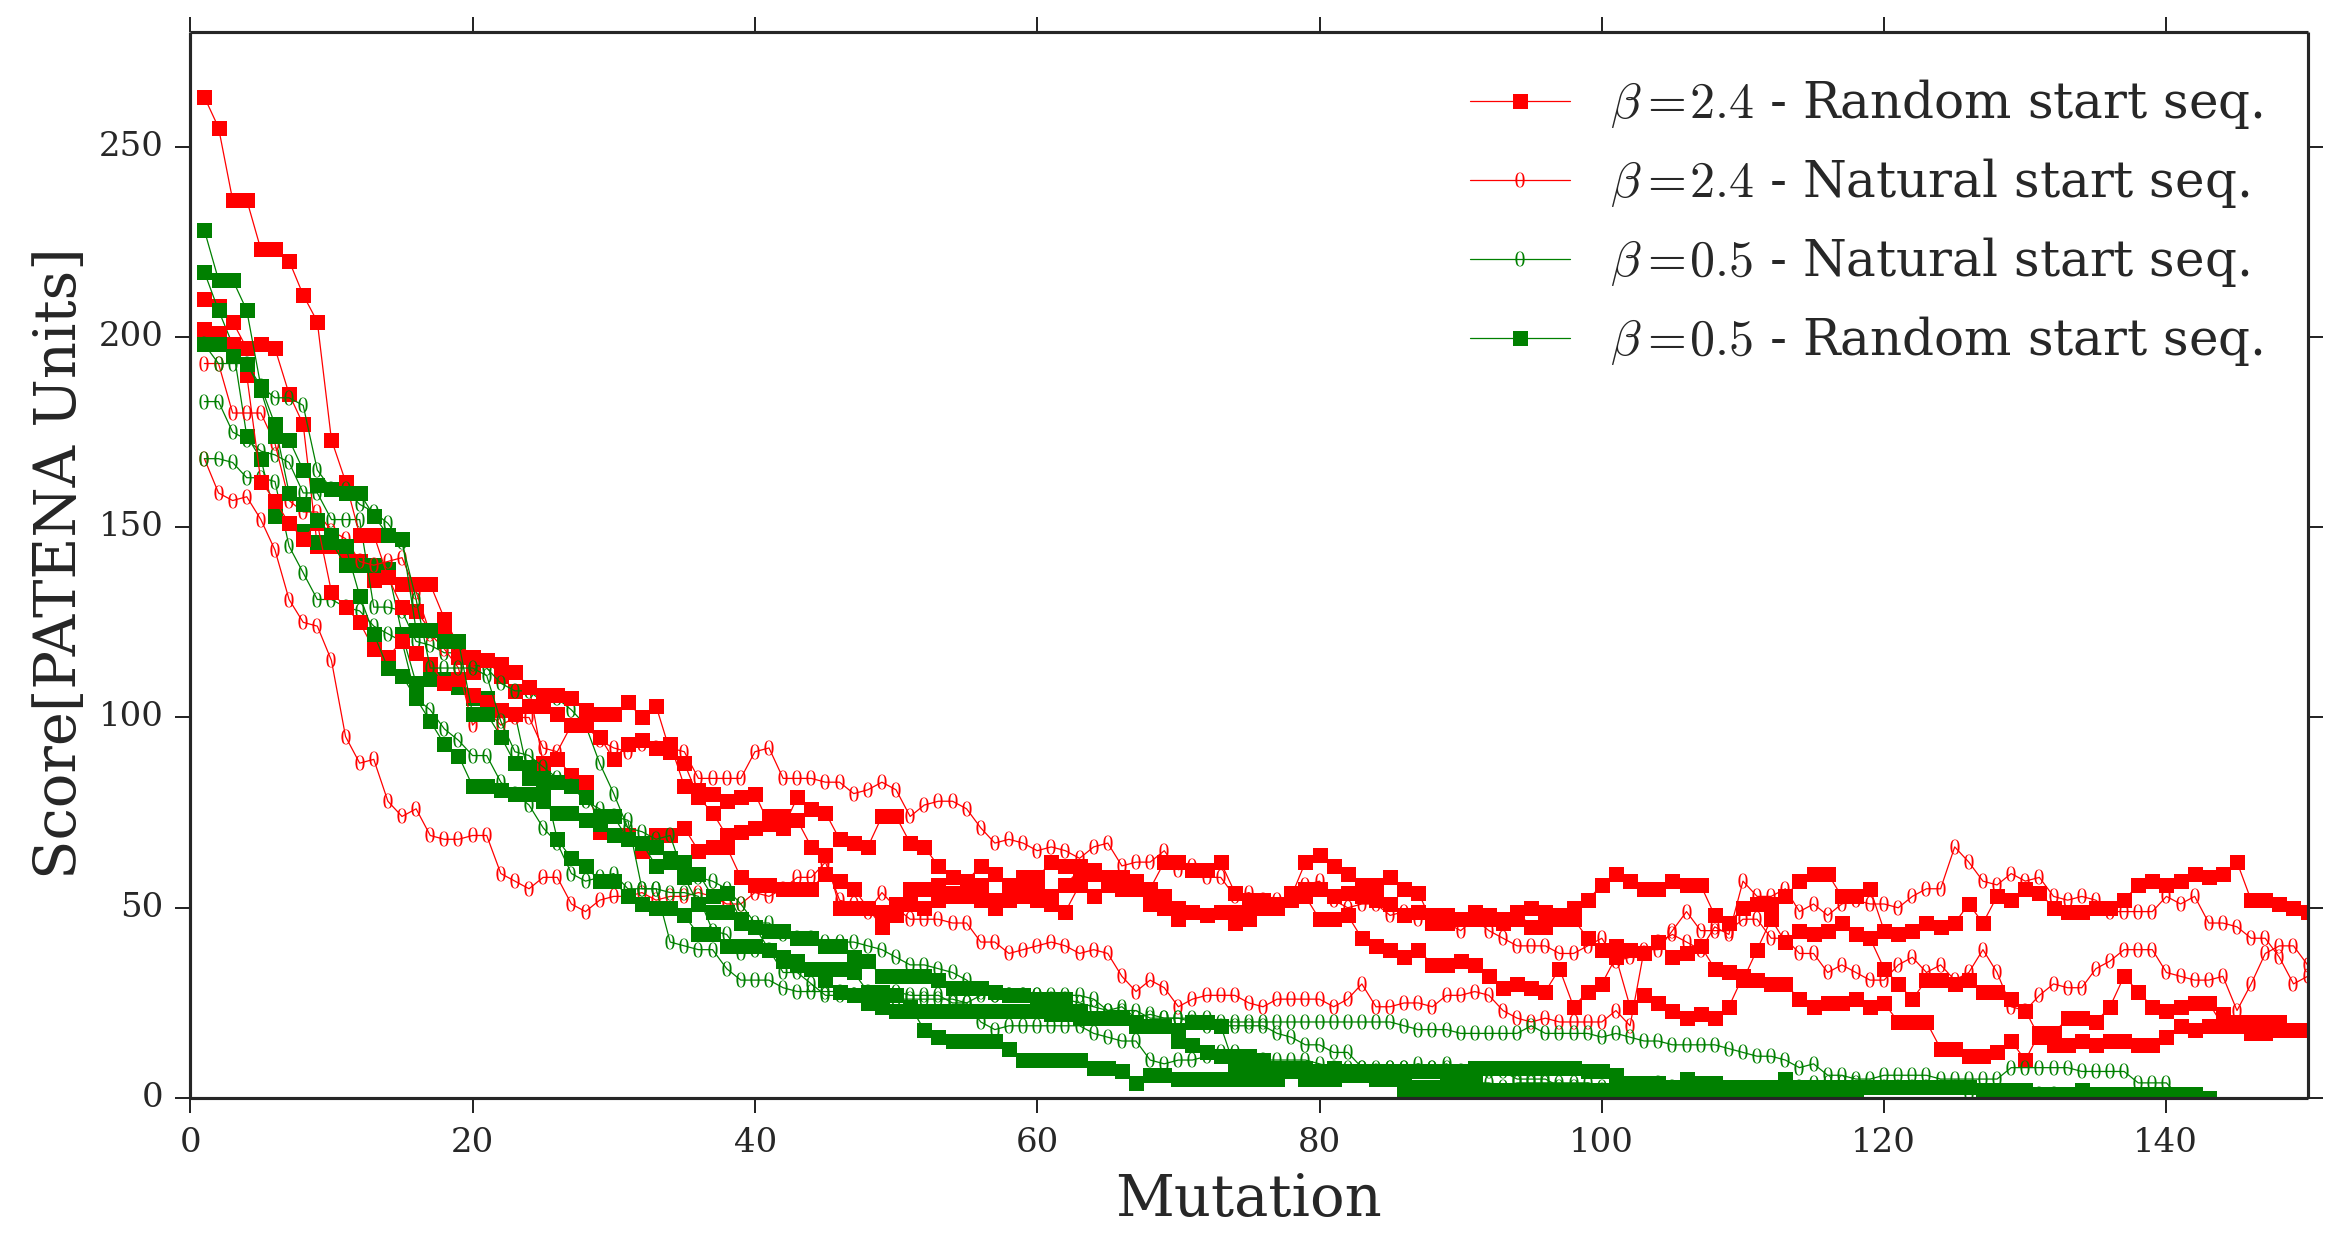
\includegraphics[width=1.1\textwidth]{img/resultados/iterationVsScore-individual.png}
    \caption{Ejecuciones individuales}
    \label{fig:scoreVsiter-a}
  \end{subfigure}
%   \hspace{20px}
  \begin{subfigure}[b]{\textwidth}
%     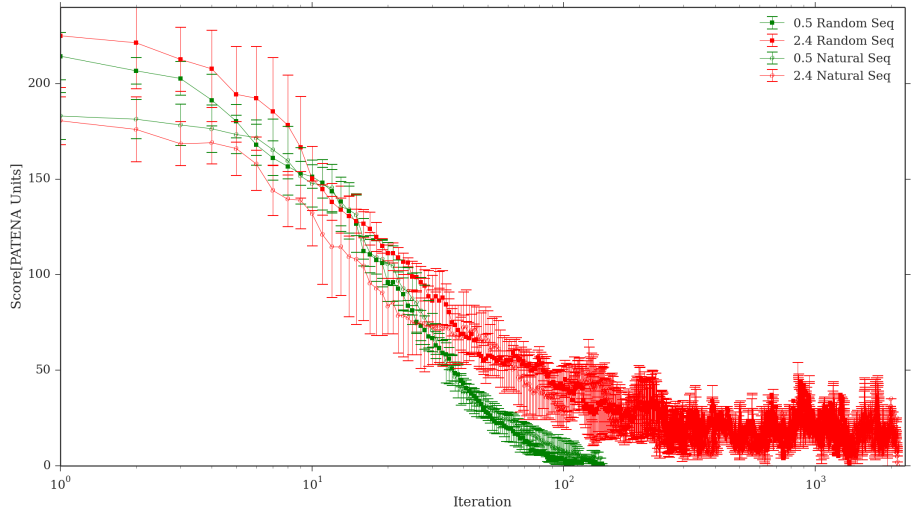
\includegraphics[width=1.15\textwidth]{img/resultados/scoreVsiter-cada1-hasta2270.png}
     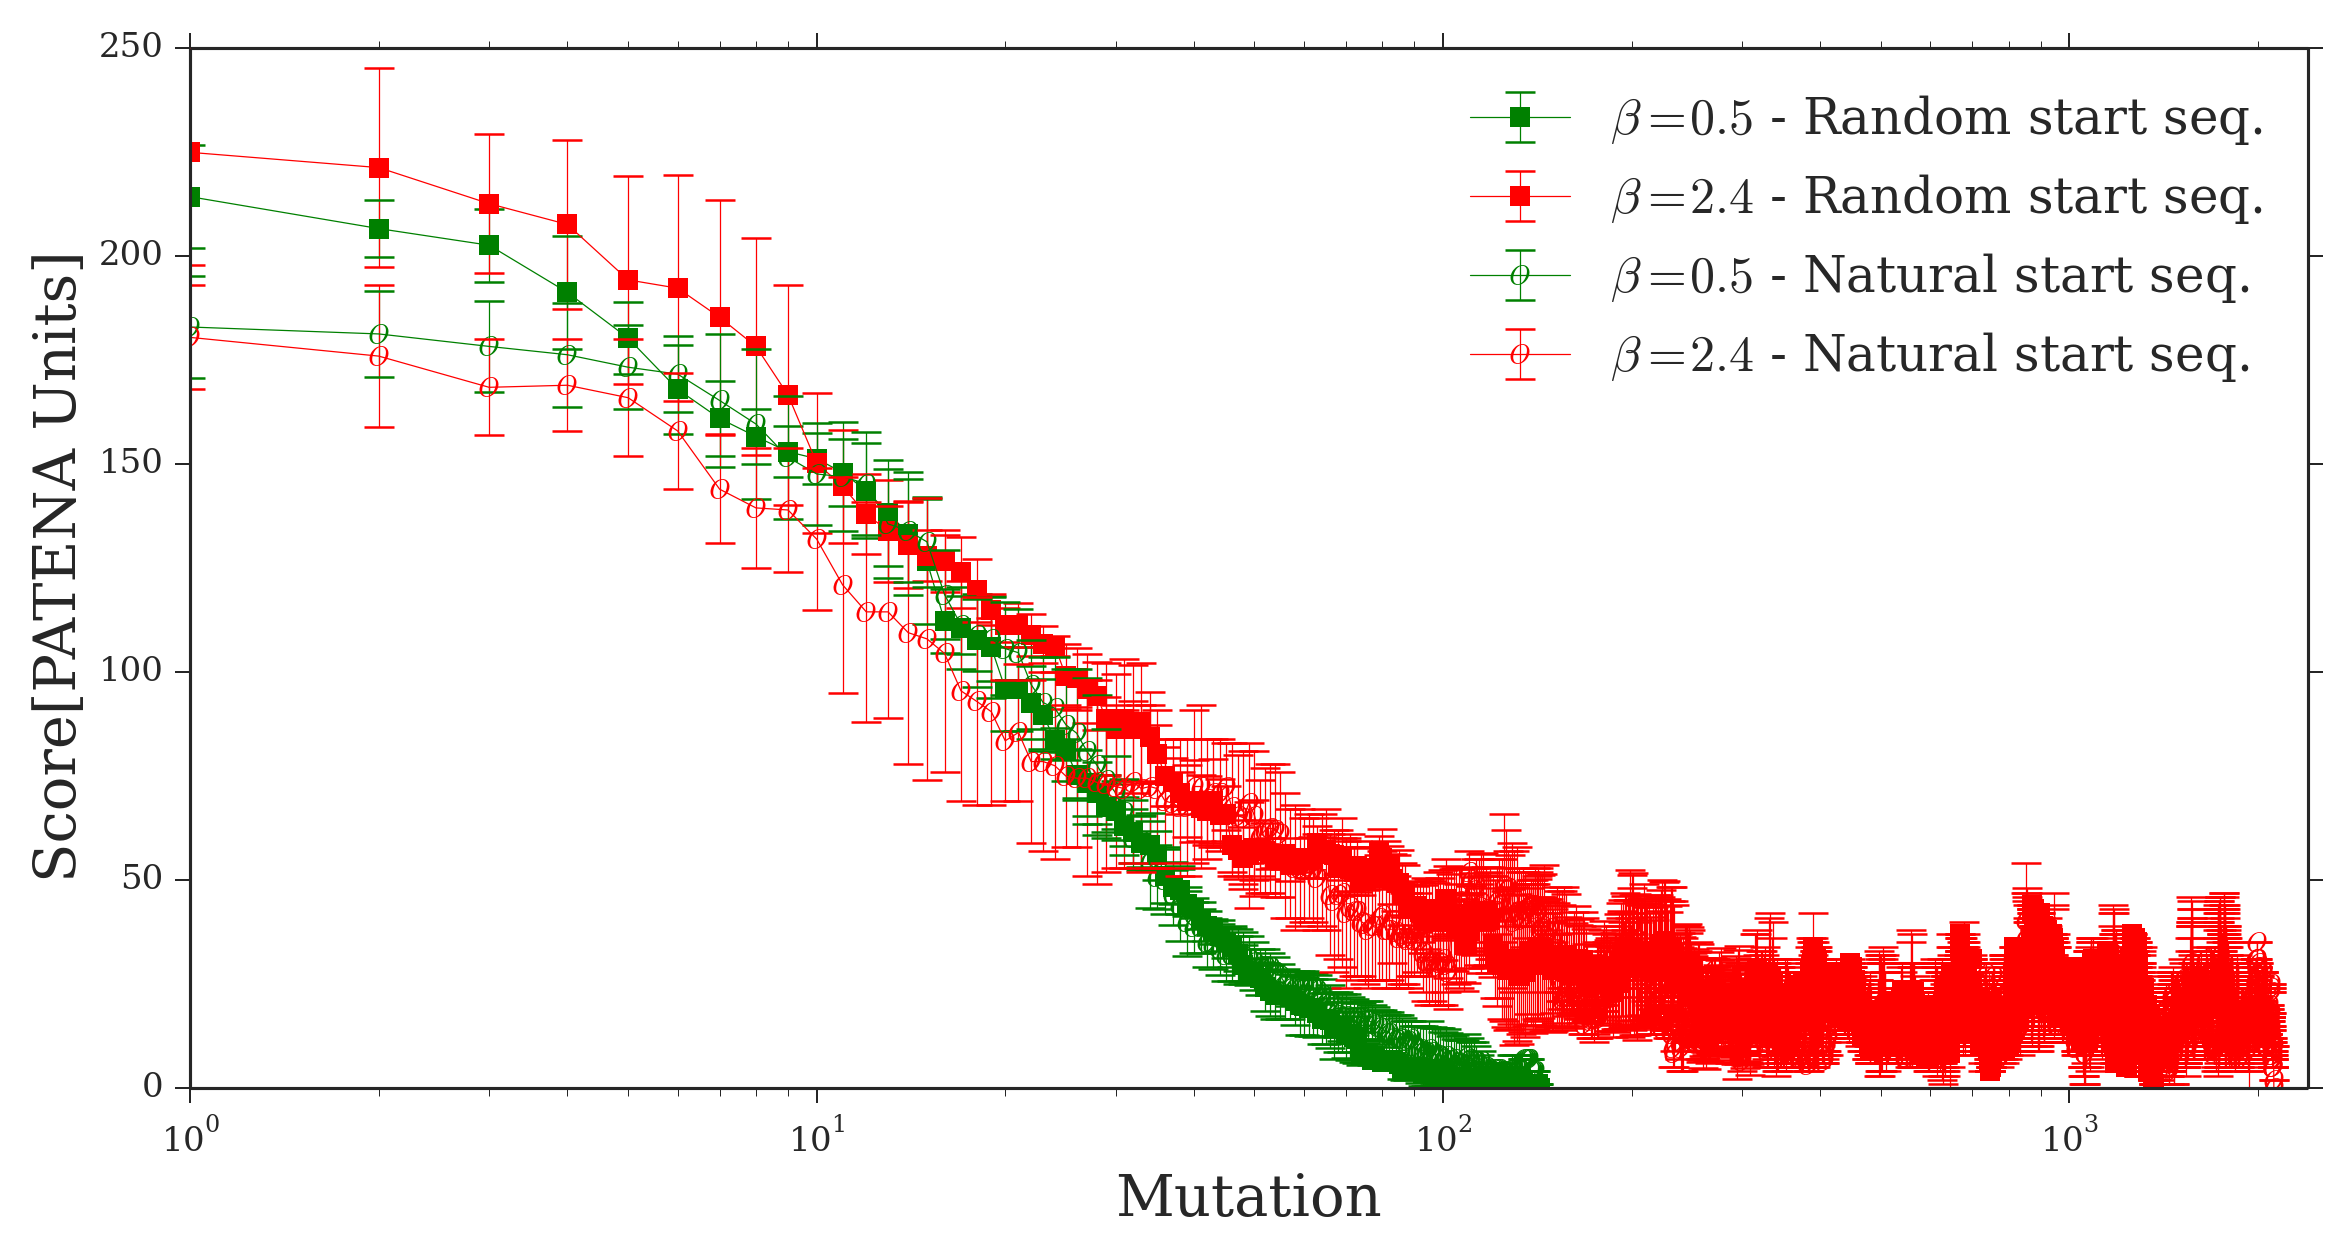
\includegraphics[width=1.1\textwidth]{img/resultados/iterationVsScore-mean.png}
    \caption{Valores medios y desviaciones}
  \label{fig:scoreVsiter-b}
  \end{subfigure}
  \caption{Puntaje asociado a cada iteración}
  \label{fig:scoreVsiter}
\end{figure}

Esta es, sin embargo, una visión muy general de la ejecución, y para tener una idea mas detallada es necesario analizar otros parámetros relevantes.
% y   MUT-ATTEMPTS vs ITERACION (MEDIAS Y StdDeV COMPLETO HASTA EL FINAL)   +  CORRIDAS INDIVIDUALES
En el gráfico \ref{fig:mutAttemptsVsite} se muestra el número de intentos de mutación asociado a cada valor de $\beta$.
Nuevamente se muestran los valores medios (y sus desviaciones correspondientes) en el gráfico \ref{fig:mutAttemptsVsite-b}, y el detalle de las ejecuciones individuales (gráfico \ref{fig:mutAttemptsVsite-a}).
Vemos que el reducido número de iteraciones que resulta de un valor bajo de $\beta$ se produce a costa de una cantidad más elevada de intentos de mutaciones, es decir, se evalúa una mayor cantidad de posibles mutaciones hasta 
que eventualmente una sea aceptada, lo que representa la dificultad del camino hacia el valor mínimo buscado. 
Esta condición se incrementa en las iteraciones cercanas al fín de la ejecución, que se corresponden con los valores más bajos de puntaje(cercanos a 0). 


% \begin{figure} 
% \advance\leftskip-2cm
% \subfigure[Ejecuciones individuales]{\label{fig:mutAttemptsVsite-a}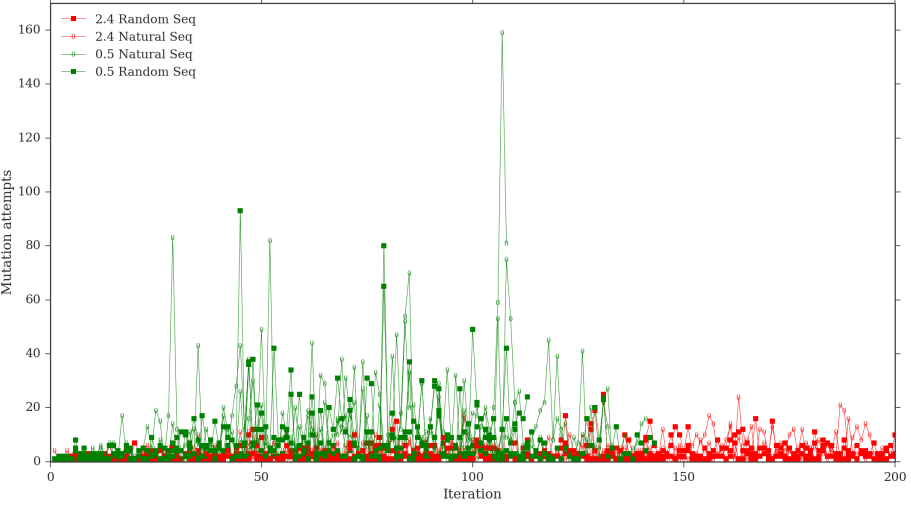
\includegraphics[width=1.15\textwidth]{img/resultados/individuales-mutAt-vs-iter-hasta200.png}}
% \subfigure[Valores medios y desviaciones]{\label{fig:mutAttemptsVsite-b}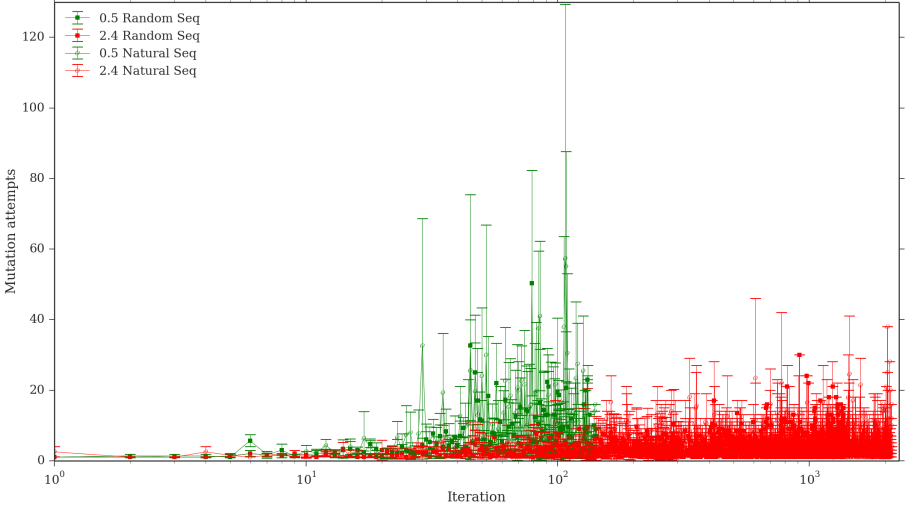
\includegraphics[width=1.15\textwidth]{img/resultados/mutAttemptsVsite-cada1-hasta2270.png}}
% \caption{Dependencia del número de intentos de mutación con la iteración}
% \label{fig:mutAttemptsVsite}
% \end{figure}


\begin{figure}[htbp]
\advance\leftskip-1.5cm
  \begin{subfigure}[b]{\textwidth}
%     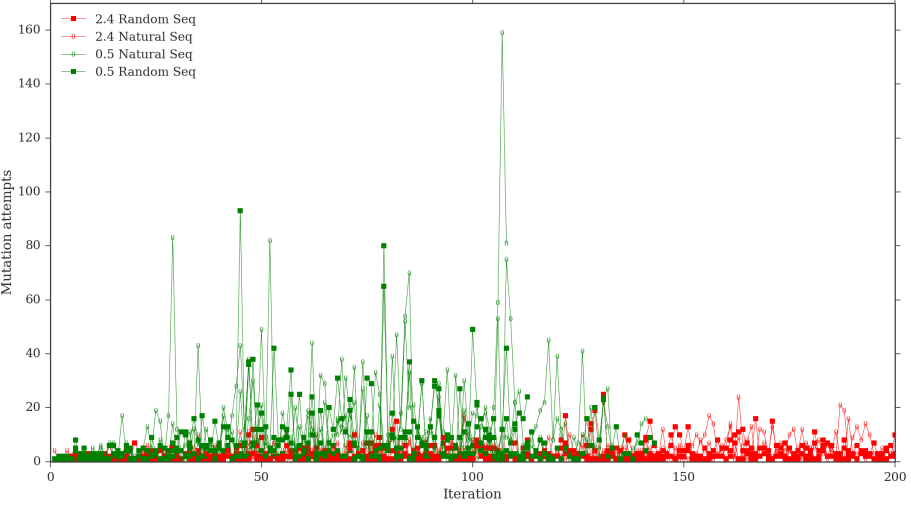
\includegraphics[width=1.15\textwidth]{img/resultados/individuales-mutAt-vs-iter-hasta200.png}
    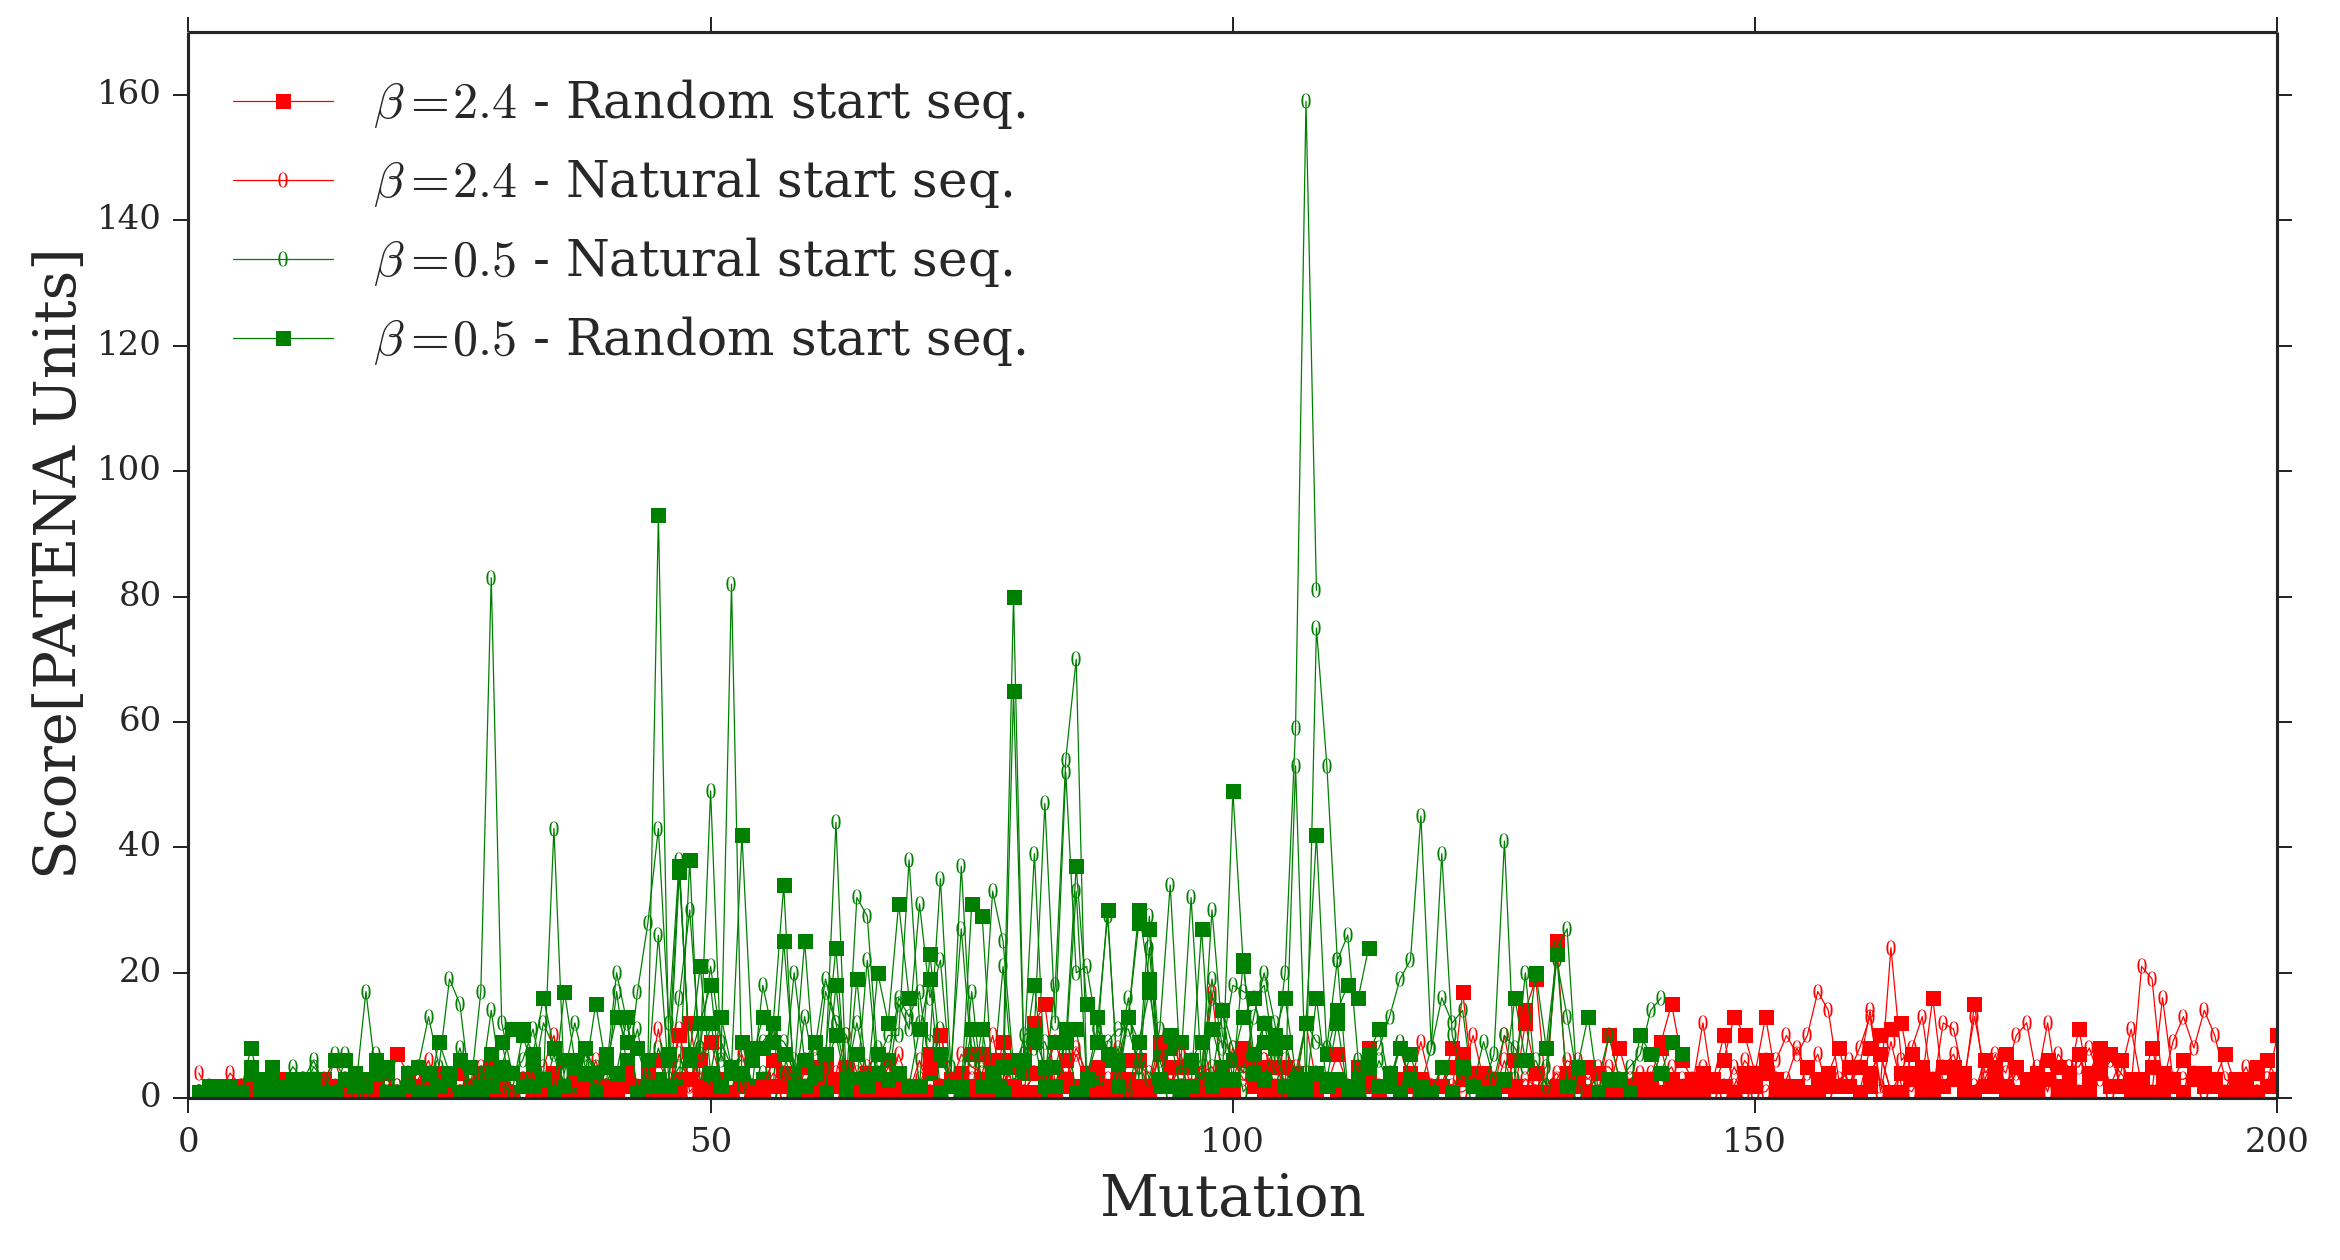
\includegraphics[width=1.1\textwidth]{img/resultados/iterationVsMutAttempts-individual.png}
    \caption{Ejecuciones individuales}
    \label{fig:mutAttemptsVsite-a}
  \end{subfigure}
%   \hspace{20px}
  \begin{subfigure}[b]{\textwidth}
%     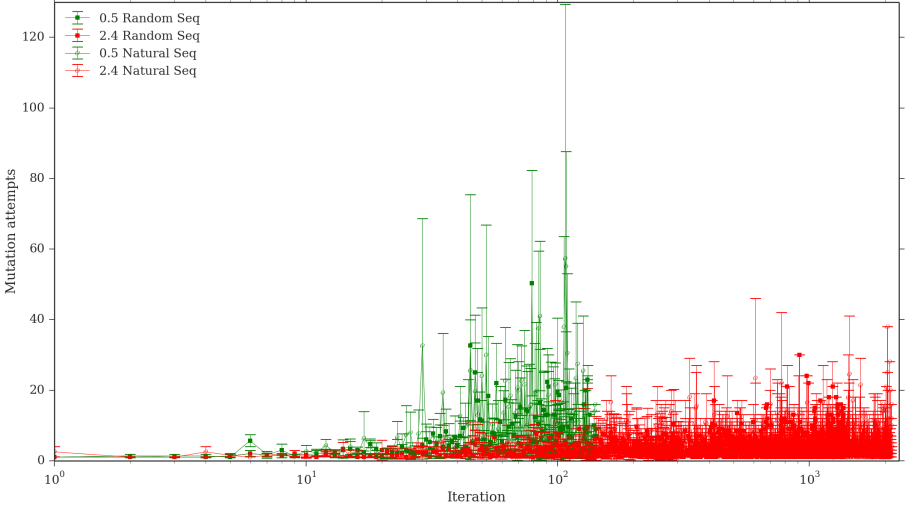
\includegraphics[width=1.15\textwidth]{img/resultados/mutAttemptsVsite-cada1-hasta2270.png}
      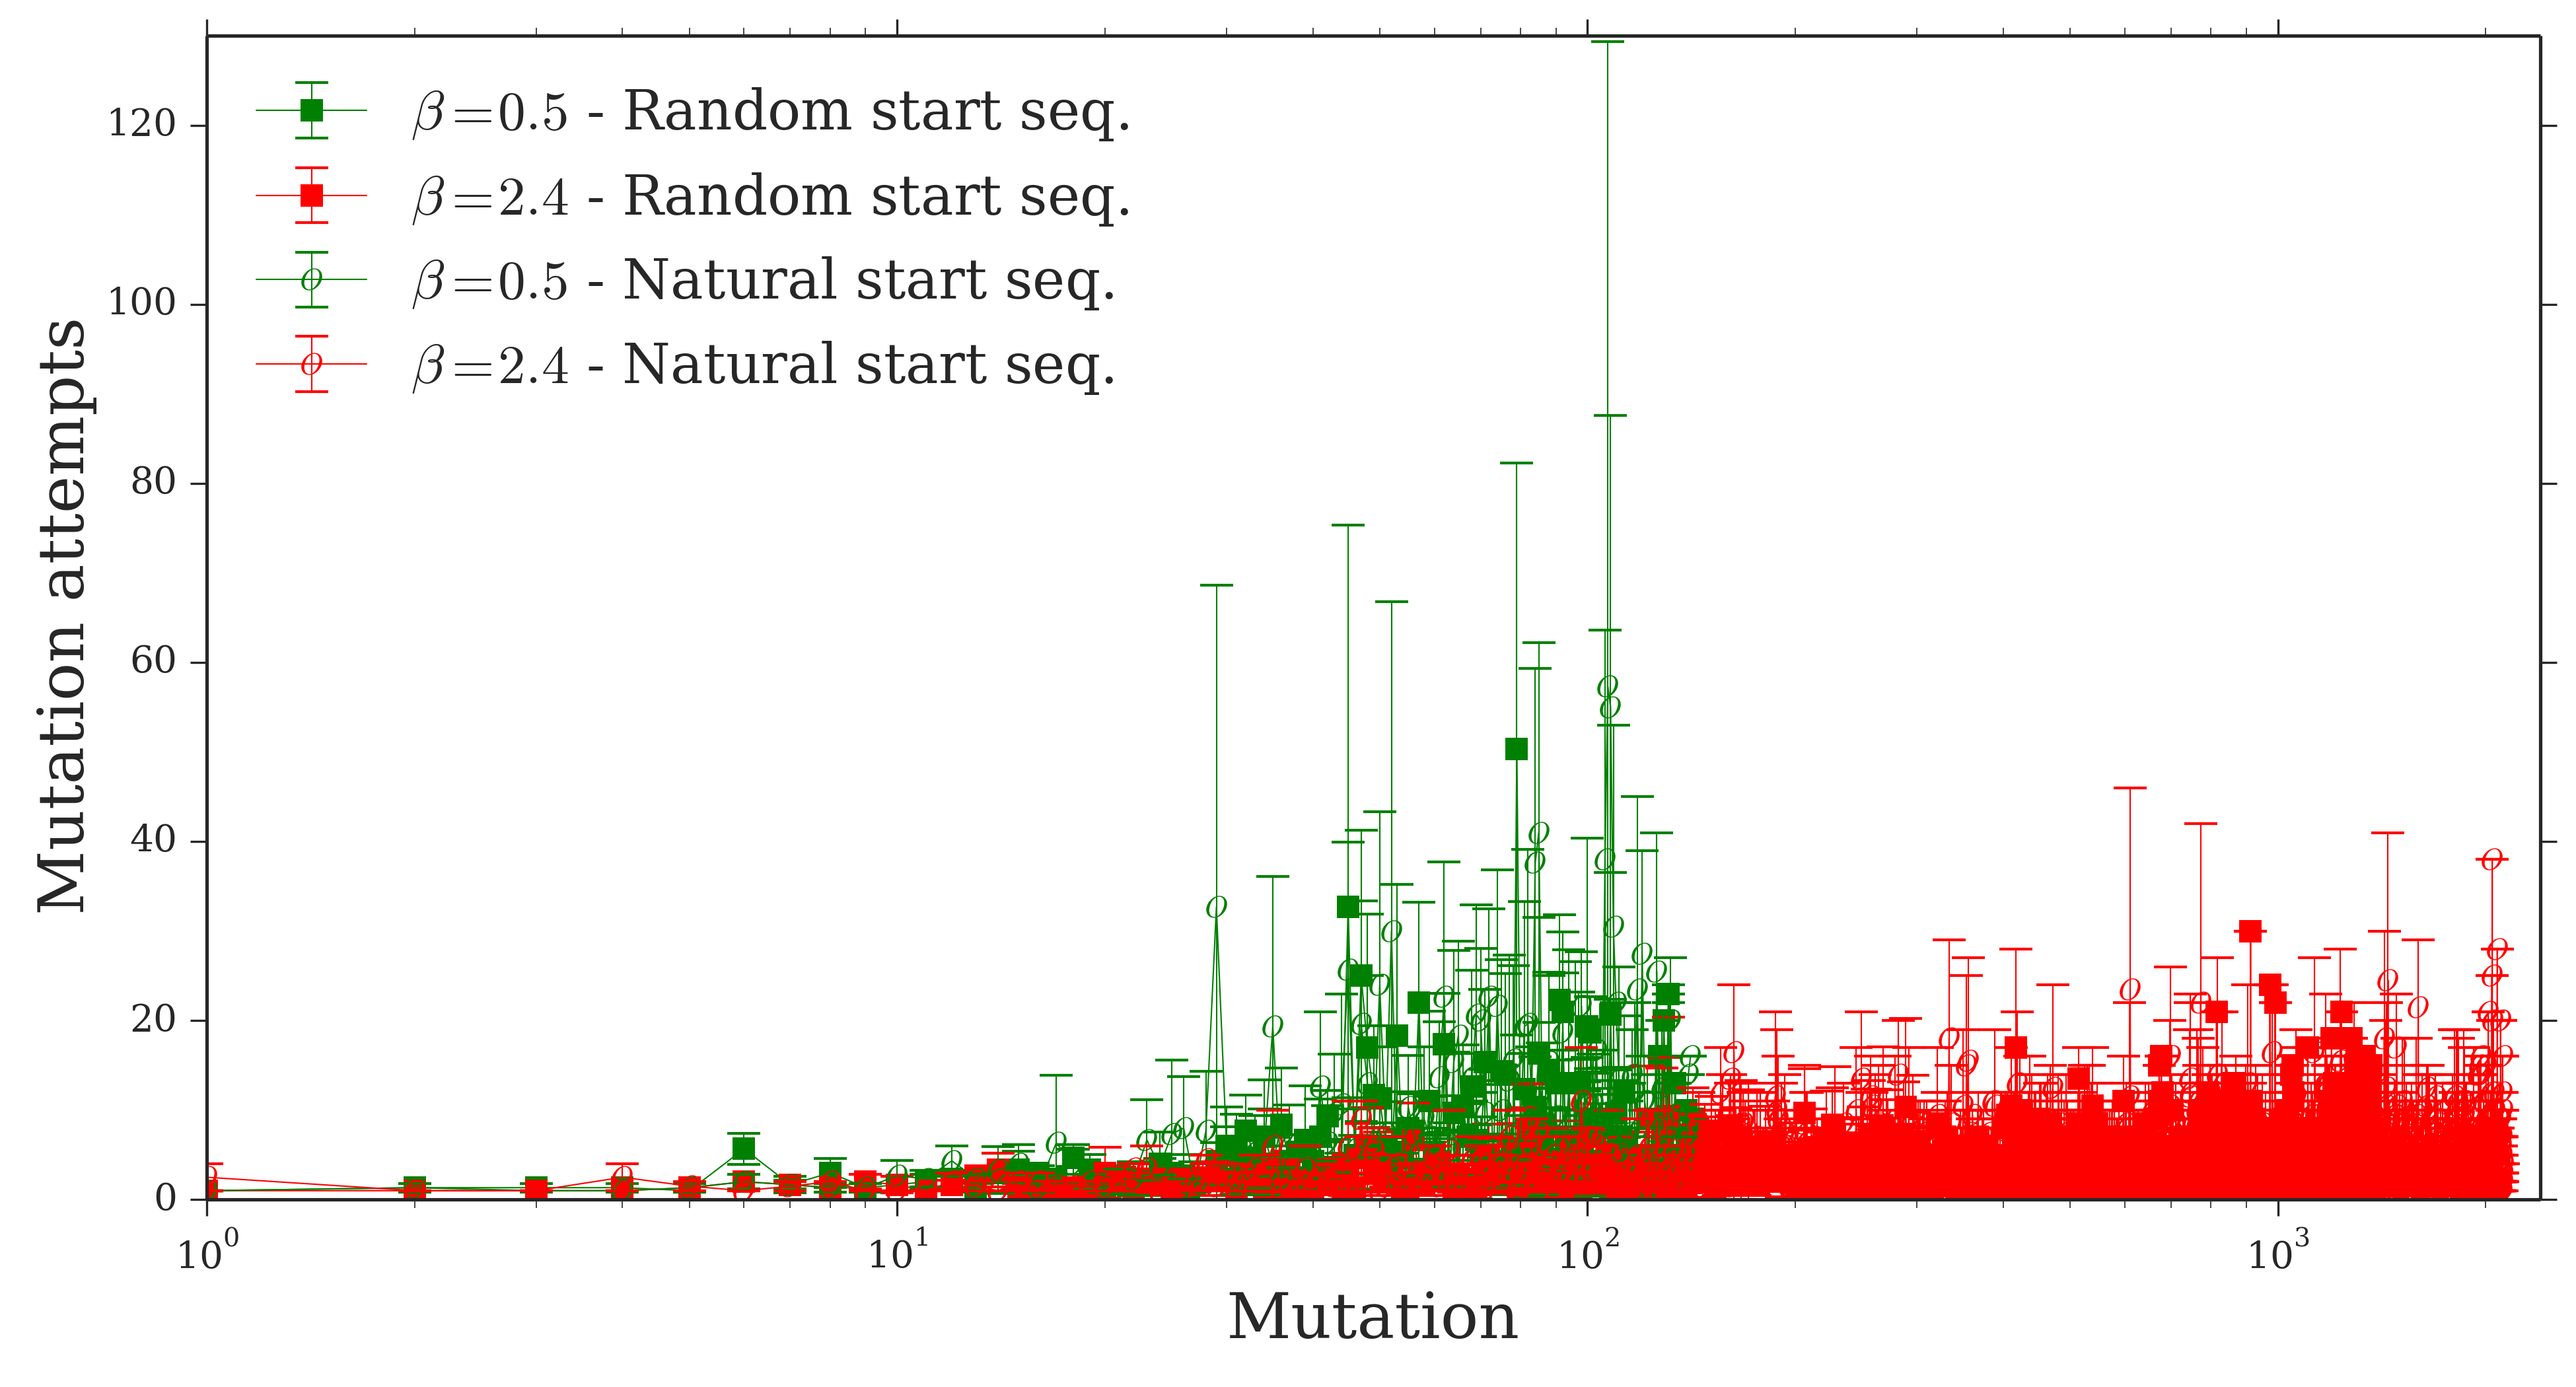
\includegraphics[width=1.1\textwidth]{img/resultados/iterationVsMutAttempts-mean.png}
    \caption{Valores medios y desviaciones}
  \label{fig:mutAttemptsVsite-b}
  \end{subfigure}
  \caption{Dependencia del número de intentos de mutación con la iteración}
  \label{fig:mutAttemptsVsite}
\end{figure}

Sin embargo, no sabemos como estos intentos de encontrar mejores mutaciones afectan a la optimalidad de la búsqueda global.
% Todavía no sabemos las implicancias de realizar esta cantidad de intentos de mutacion sobre la búsqueda.
Para conocer cual es el rango(o valor) óptimo de $\beta$ utilizamos como variable de evaluación al tiempo de ejecución, 
el cual es directamente proporcional a la cantidad total de mutaciones aceptadas que se necesitan y la cantidad de mutaciones que se intentan.
Por lo tanto, la estimación del valor de $\beta$ que provea un menor tiempo de ejecución nos permite conocer cual es el valor que provee un correcto balance entre la exploración y la explotación de la superficie.
La evaluación realizada implicó evaluar el tiempo de ejecución para distintos valores de beta en el rango 0.1-2.5.
Puntualmente se analizan los valores en el conjunto (0.1, 0.5, 1.0, 1.5, 2.0, 2.3, 2.5). 
Se realizaron 6 ejecuciones para cada valor de $\beta$ analizado, de las cuales 3 se realizan a partir de secuencias definidas(obtenidas de proteínas naturales) y otras 3 a partir de secuencias generadas aleatoriamente.
En todos los casos con una longitud de 50 residuos.

En la figura \ref{fig:beta-vs-time} se muestran los tiempos medios asociados a cada conjunto de evaluaciones.
En primer lugar vemos que no hay una diferencia significativa constante entre las ejecuciones que inician a partir de secuencias naturales y las que lo hacen a partir de secuencias aleatorias.
% Al parecer, si bien las primeras pueden tener valores de score mayore
Por otro lado, se ve que el tiempo de ejecución es altamente variable para la mayoria de los valores de $\beta$.
Esta alta variabilidad, que se basa en las propiedades estocásticas de la búsqueda, no permite definir un valor óptimo puntual aunque se ve que el tiempo de ejecución es significativamente mayor en el caso de beta muy grande(2.5), 
inficando que el rango óptimo de valores para $\beta$ está ubicado hacia el extremo inferior.
Aunque el rango completo 0.1-2.0 es aceptable, tomamos un valor de $\beta=1.0$, a partir de ahora, como un valor aceptado que nos permitirá realizar la ejecución en un tiempo aceptable.



\begin{figure}[htbp]
\advance\leftskip-1.2cm
% 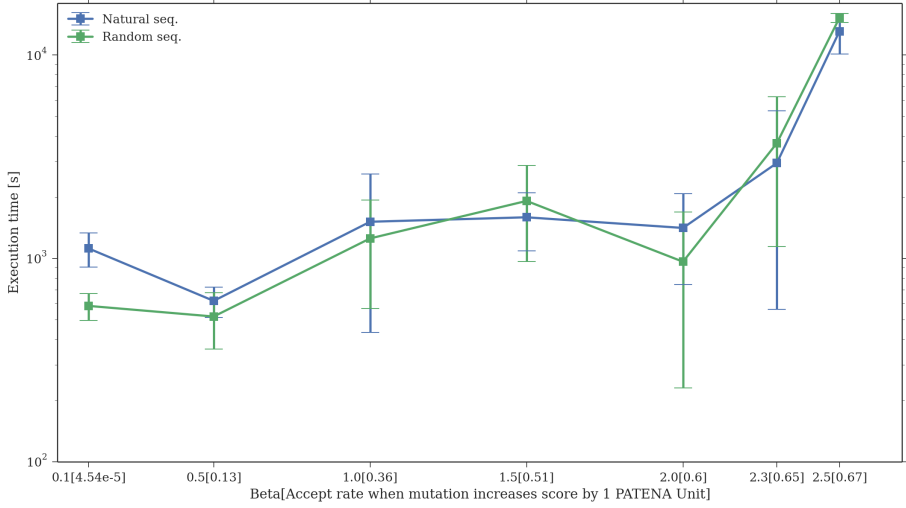
\includegraphics[width=1.1\textwidth]{img/resultados/beta-vs-time-length50-rate.png}
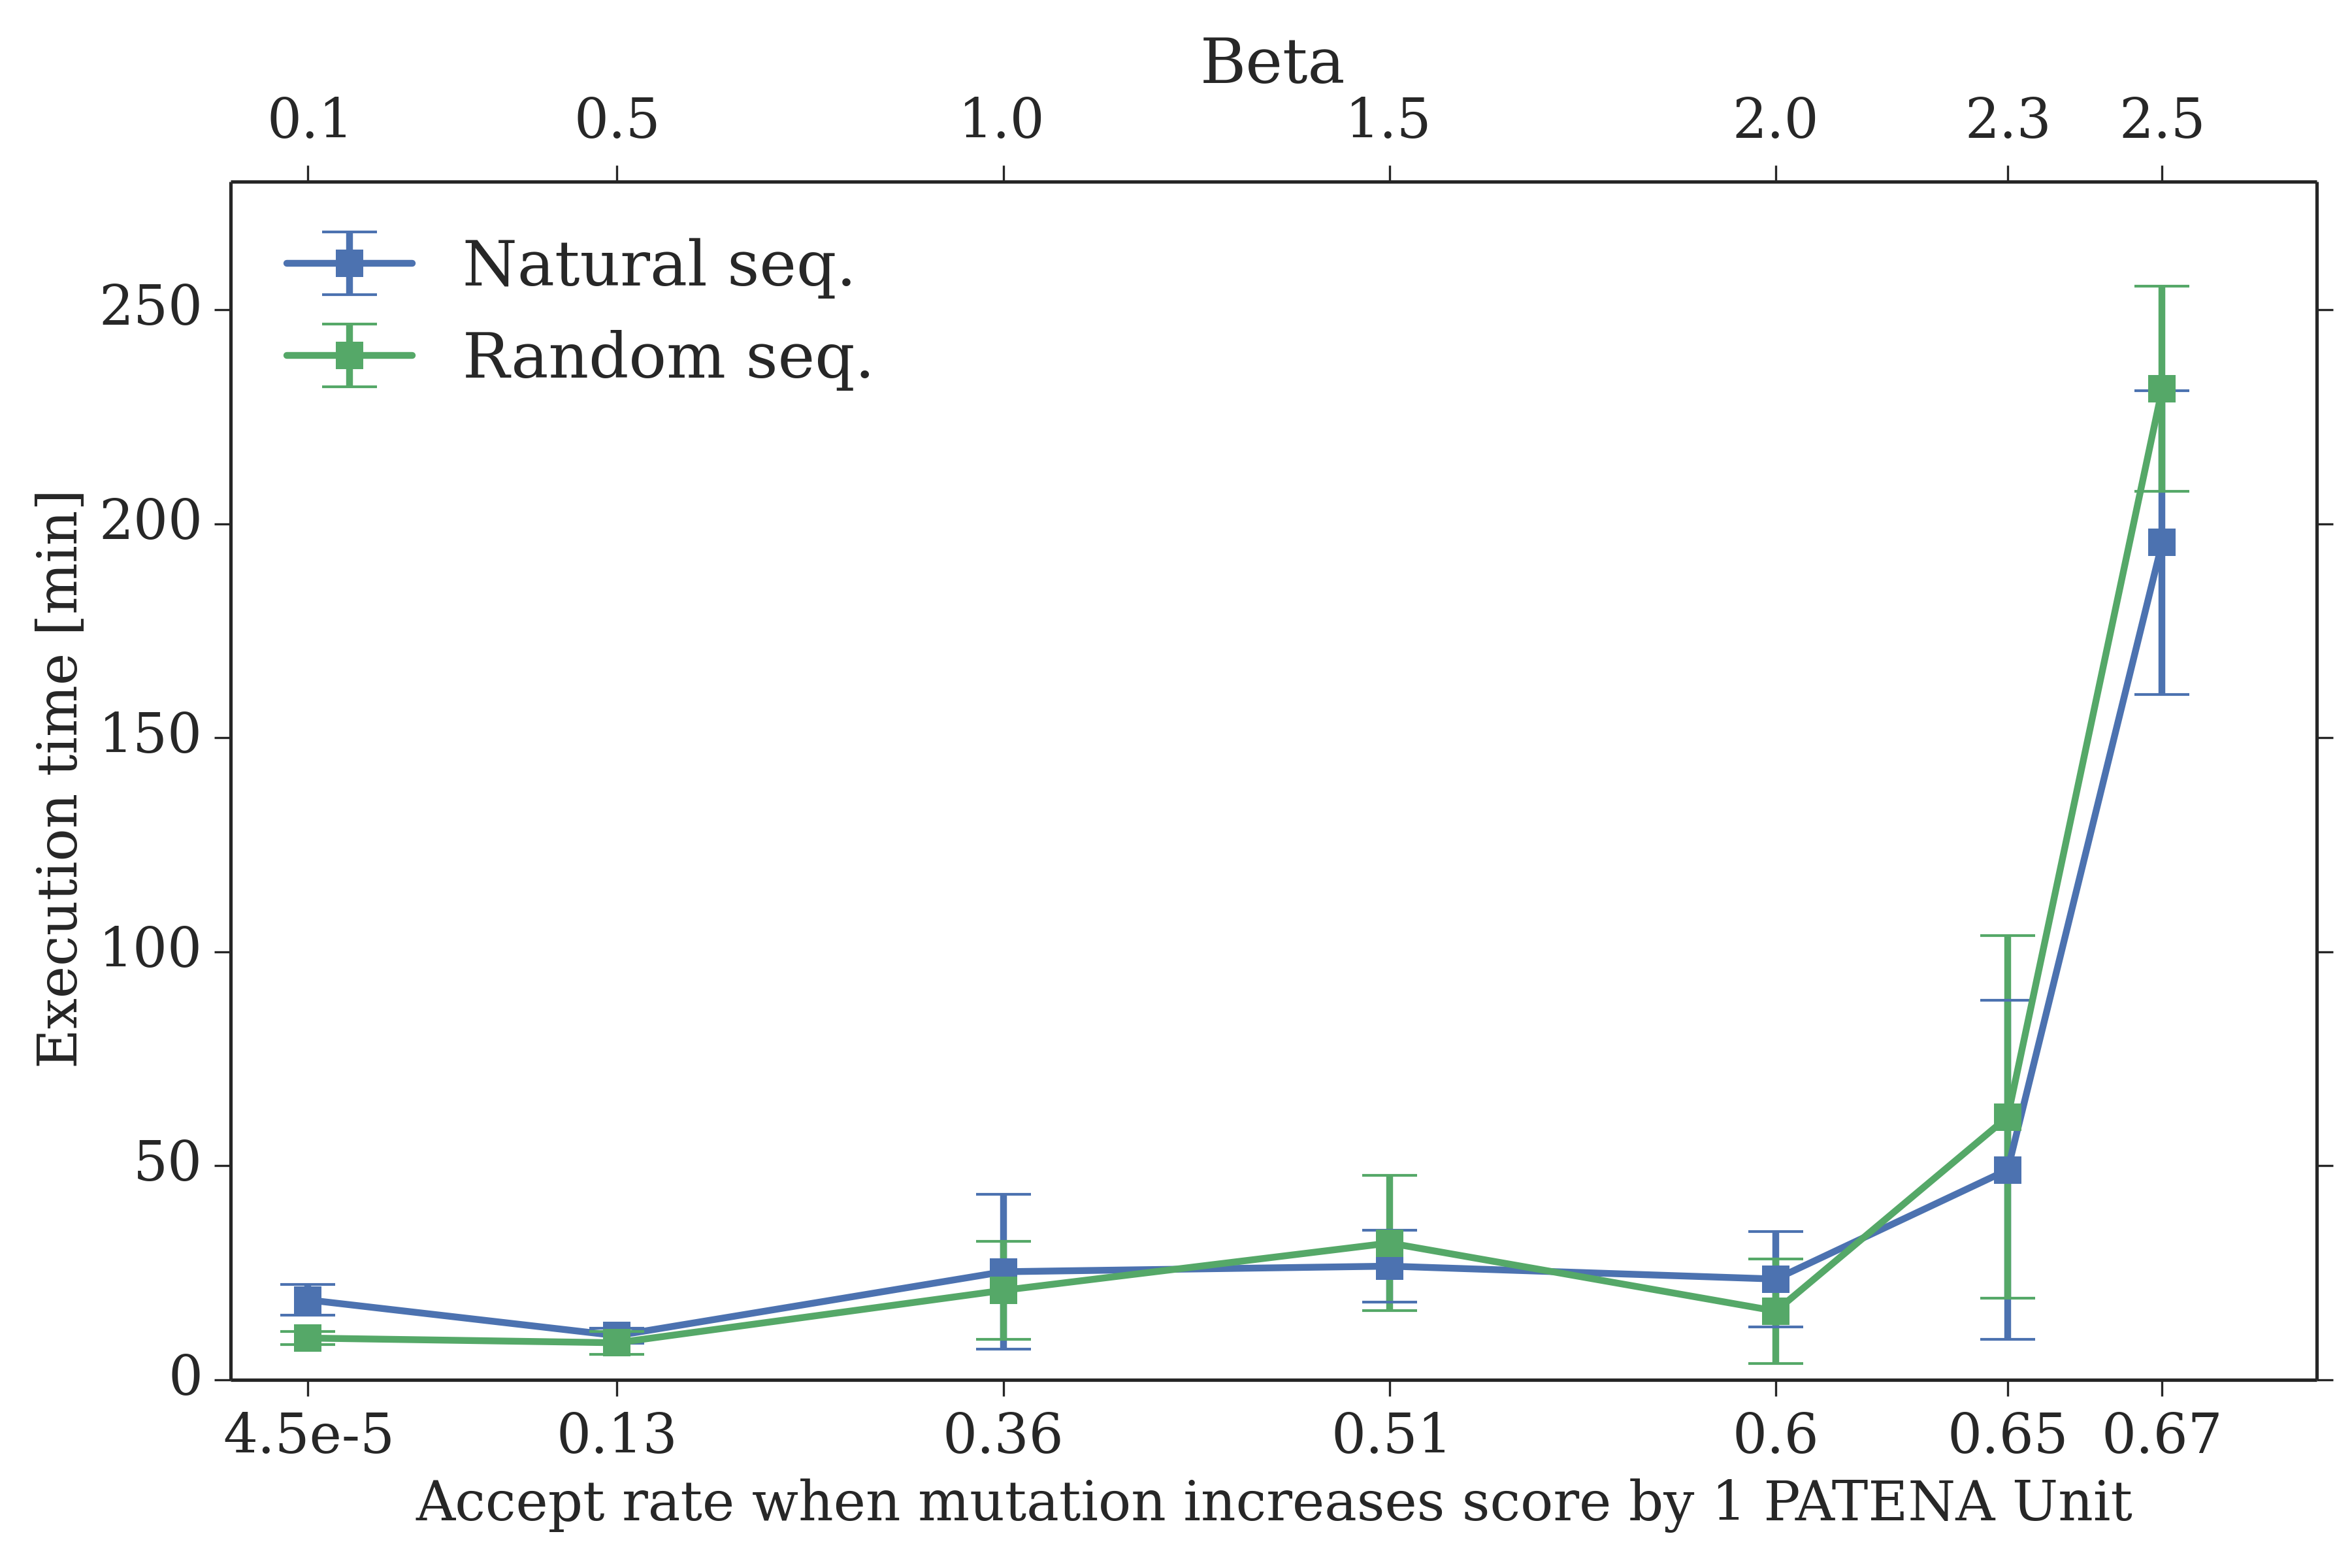
\includegraphics[width=1.1\textwidth]{img/resultados/beta-vs-time-length50-300dpi.png}
\caption{Largo de secuencia = 50}
\label{fig:beta-vs-time}
\end{figure}



\section{Tiempo de ejecución correspondiente}

% RESULTANDOS DE TIEMPO EN FUNCION DE LONGITUD
% Ahora que tenemos fijado un valor para el parámetro $\beta$ y tenemos un conjunto definido de herramientas de evaluación
Una vez definido un valor de beta que permite un balance estable entre intentos de mutación y mutaciones aceptadas, queremos saber como se traduce esto en un tiempo de ejecución concreto para distintos casos de uso de la herramienta.
Se realizan, entonces, evaluaciones del tiempo de ejecución en función de la longitud de la secuencia, lo que nos dará una idea del orden de tiempo que demoran las ejecuciones y como éste varía con la longitud.
% Utilizando los parámetros estándar, el tiempo de ejecución solo varía con la longitud de la secuencia. 
En el gráfico \ref{fig:time-vs-length} se muestran los resultados de distintas ejecuciones individuales de la aplicación, utilizando siempre el valor de $\beta$ definido previamente(1.0), pero con longitudes de secuencia variable, 
tanto para secuencias aleatorias como para secuencias iniciales naturales.

Si bien los resultados parecen indican una relación aproximadamente lineal entre la longitud de la secuencia y el tiempo de ejecución, la relevancia de estos resultados es que nos permiten 
saber que la solución es aplicable a secuencias en el rango esperado de utilización de la herramienta. 

\begin{figure}[htbp]
\centering
% 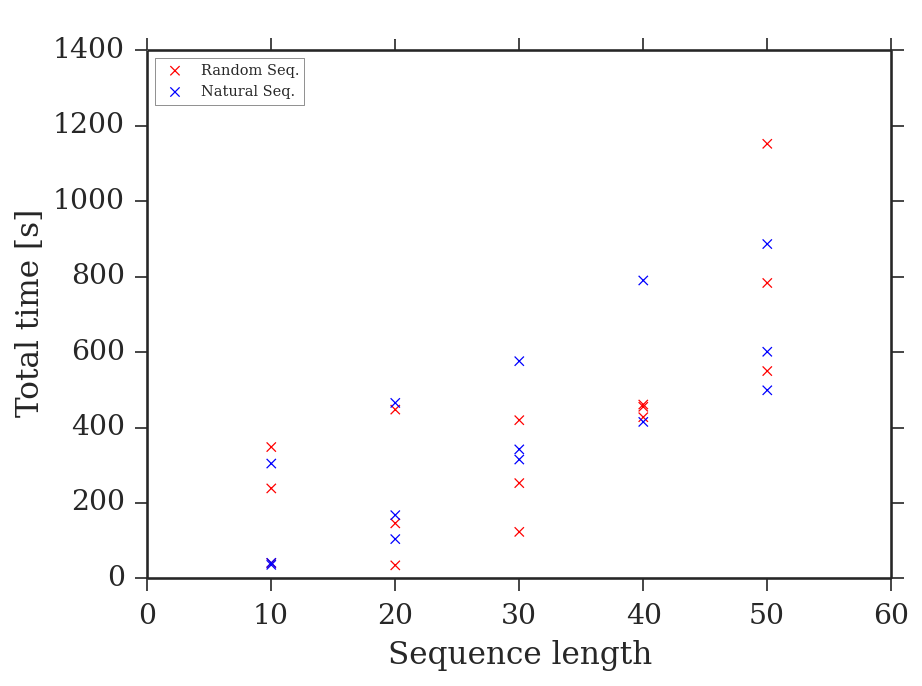
\includegraphics[width=0.8\textwidth]{img/resultados/time-vs-length-beta1.png}
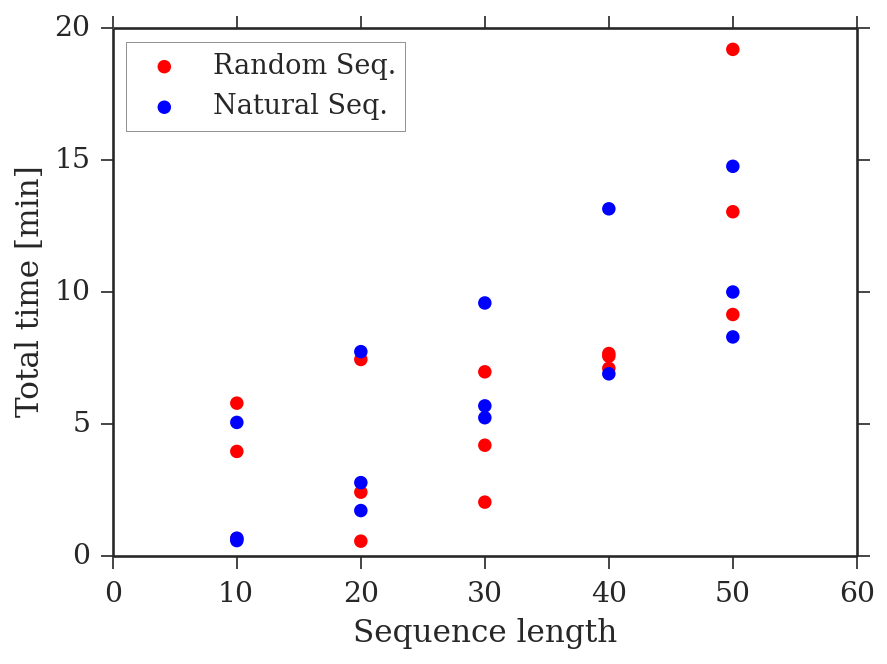
\includegraphics[width=0.8\textwidth]{img/resultados/lengthVsTime.png}
\caption{}
\label{fig:time-vs-length}
\end{figure}





\section{Análisis de diseños resultantes}

% DIVERGENCIA EN EL CONJUNTO DE RESULTADOS
Ahora que tenemos fijados todos los aspectos de ejecución del método y que efectivamente podemos obtener, en un tiempo aceptable, secuencias que cumplen con requerimientos definidos, nos centraremos en 
conocer más acerca de los diseños resultantes.
Por definición del método, sabemos que los resultados tendrán las propiedades positivas buscadas y no tendrán las características negativas pero, hasta el momento, no sabemos nada más acerca de los diseños que se pueden obtener.
Teniendo en cuenta los fundamentos del método, que describen a las secuencias buscadas como un conjunto amplio y complejo, y las características no determinísticas del método,
es posible pensar que debería existir al menos cierta diversidad entre los resultados, aún cuando se comparen los resultados de ejecuciones que comienzan en una misma secuencia inicial.

Hasta el momento vimos el proceso de ejecución analizando de forma abstracta el número de iteraciones, sin tener en cuenta sobre que posiciones se aplicaban,
sin embargo, la diversidad resultante de la búsqueda dependerá fuertemente del número y distribución de mutaciones que se aplican sobre la secuencia inicial.
Para analizar estos aspectos se realizaron un total de 74 ejecuciones independientes a partir de una misma secuencia inicial(\texttt{MALWMRLLPLLALLALWGPDPAAAFVNQHL}).
En primer lugar se analizaron los porcentajes de mutación para cada posición de la secuencia, los cuales se muestran en la figura \ref{fig:mutationPerSite}.
Si bien no hay ninguna diferencia significativa en el patrón de mutaciones, las 4 posiciones que presentan el menor porcentaje medio de mutaciones(residuos 9,18,19,21),
se corresponden con residuos de Prolina y Glicina.
Como vimos en el capítulo 1, estos son los residuos más encontrados en linkers tanto naturales como artificiales debido a sus propiedades fisicoquímicas caracterísicas.

\begin{figure}[htbp]
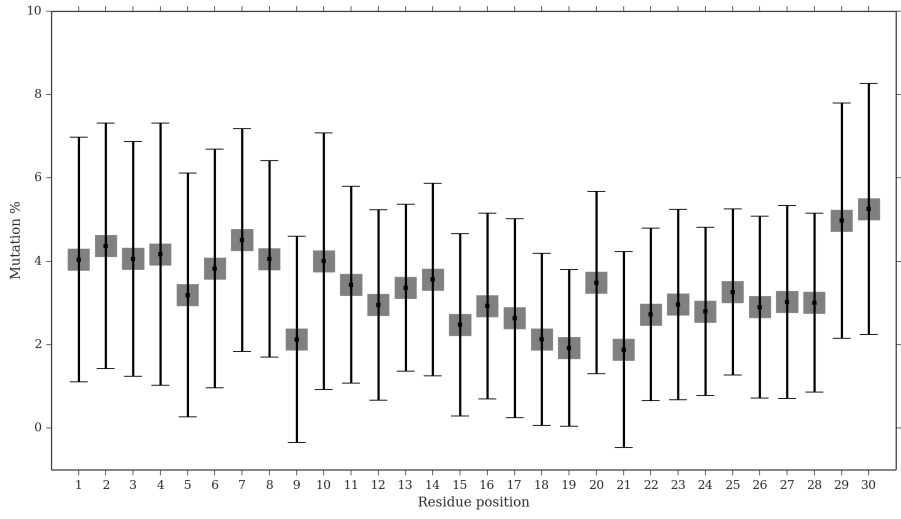
\includegraphics[width=\textwidth]{img/resultados/mutationsPerPosition.png}
\caption{Procentaje de mutaciones medio para cada posición en 74 corridas individuales}
\label{fig:mutationPerSite}
\end{figure}


% ANALISIS DE LA IDENTIDAD SECUENCIAL
Luego se analizaron las características secuenciales de este conjunto de resultados, evaluando el procentaje de identidad secuencial entre estos y con la secuencia inicial (figura \ref{fig:identity}). 

% \begin{figure}[htbp]
% % \advance\leftskip-2cm
% \centering
% \subfigure[h][Identidad entre las secuencias resultantes(74) y la secuencia inicial]{\label{fig:identity-a}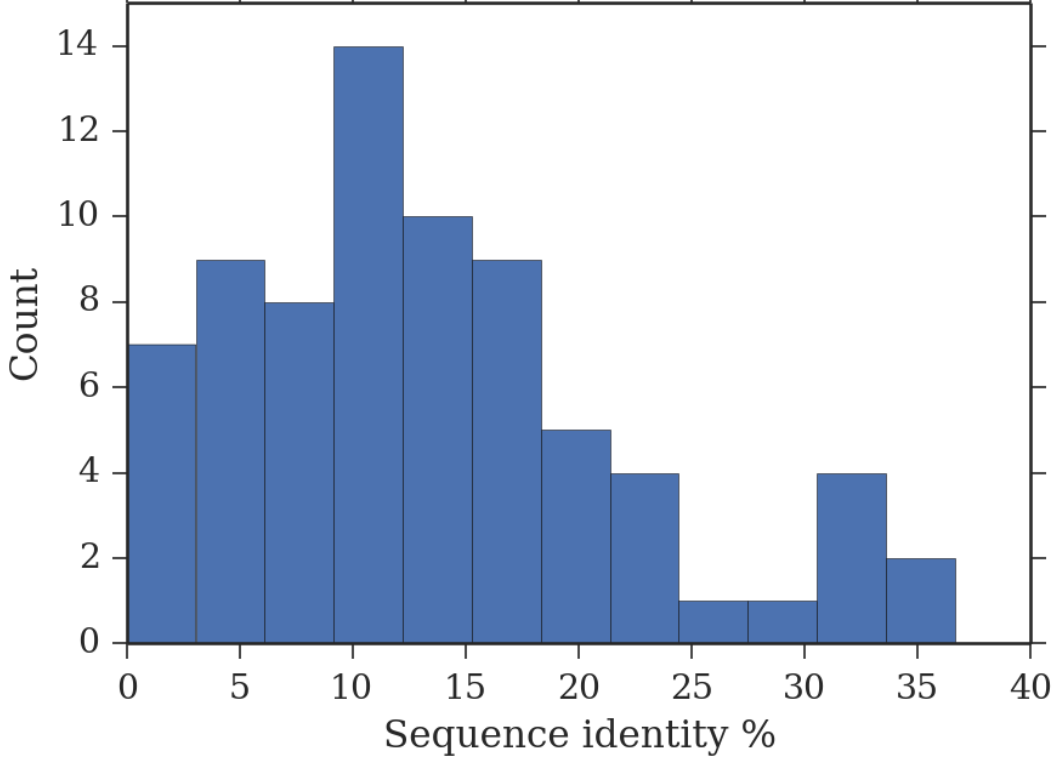
\includegraphics[width=0.5\textwidth]{img/resultados/againstStartSeq-74.png}}
% \subfigure[h][Identidad entre cada par posible de secuencias resultantes(74*74)]{\label{fig:identity-b}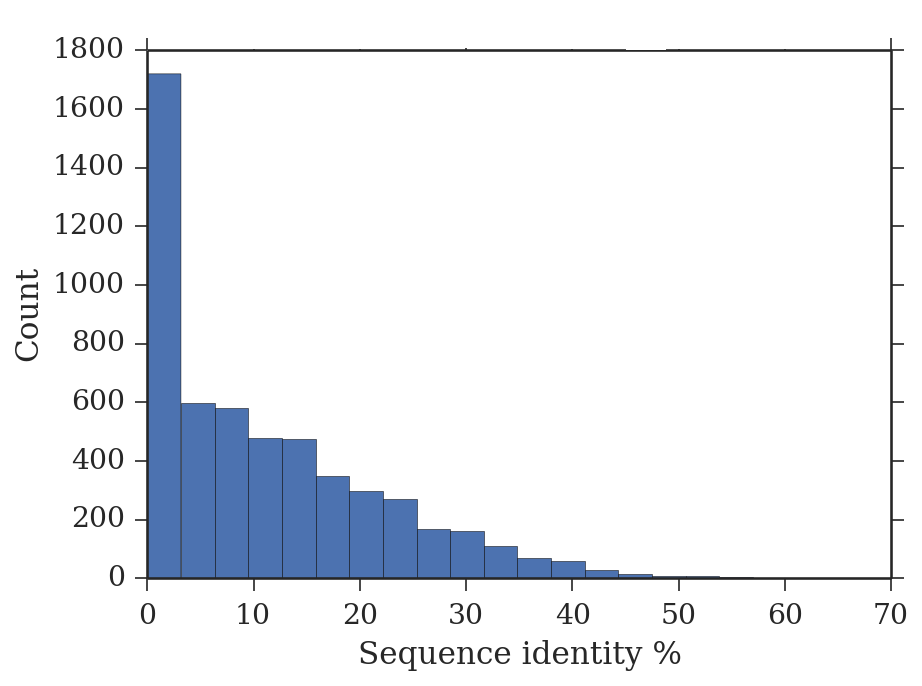
\includegraphics[width=0.5\textwidth]{img/resultados/againstAll-74-borrado.png}}
% \caption{Histograma de identidad de las secuencias resultantes}
% \label{fig:identity}
% \end{figure}



\begin{figure}[htbp]
% \advance\leftskip-1.2cm
  \begin{subfigure}[b]{200px}
%     \caption{}
%     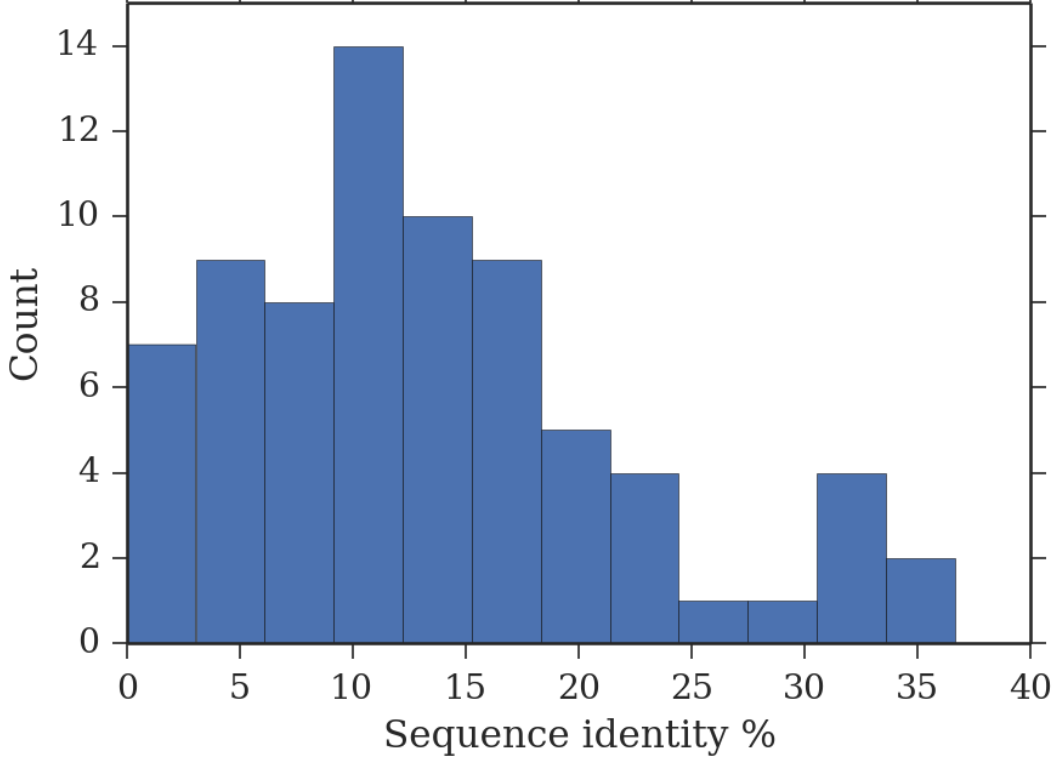
\includegraphics[width=240px]{img/resultados/againstStartSeq-74.png}
  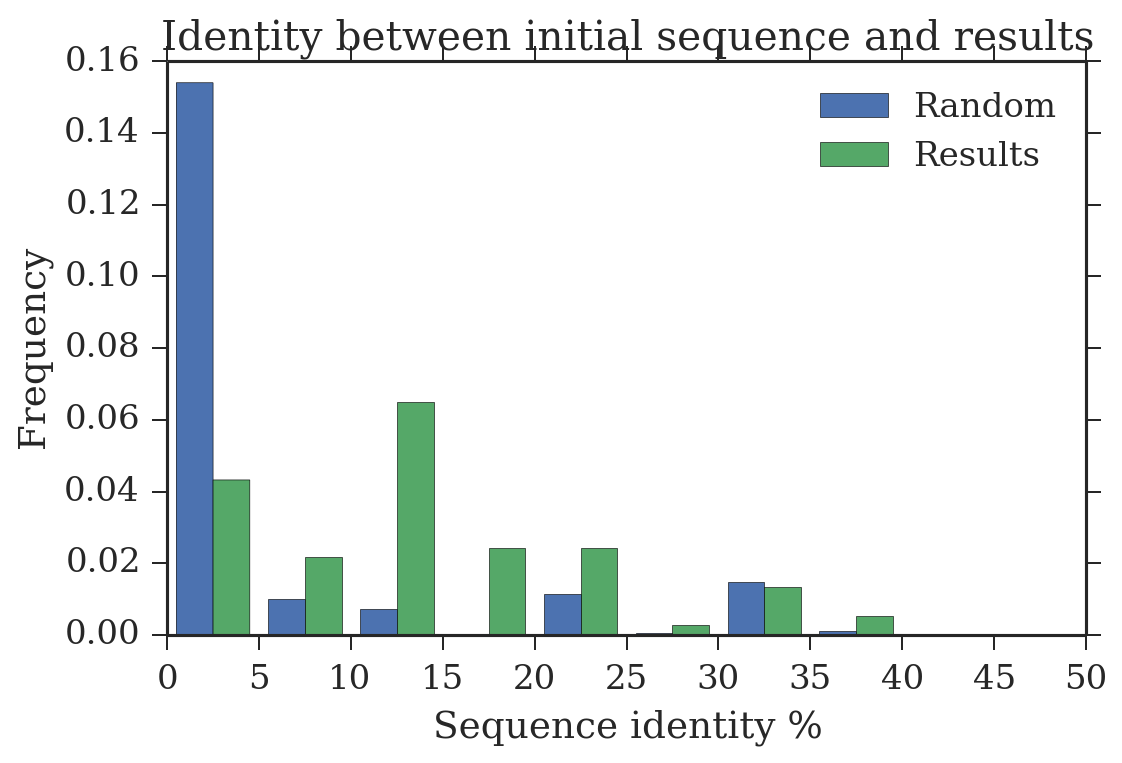
\includegraphics[width=240px,height=185px]{img/resultados/againstInitial-random.png}
    \label{fig:identity-a}
  \end{subfigure}
  \hspace{30px}
  \begin{subfigure}[b]{200px}
    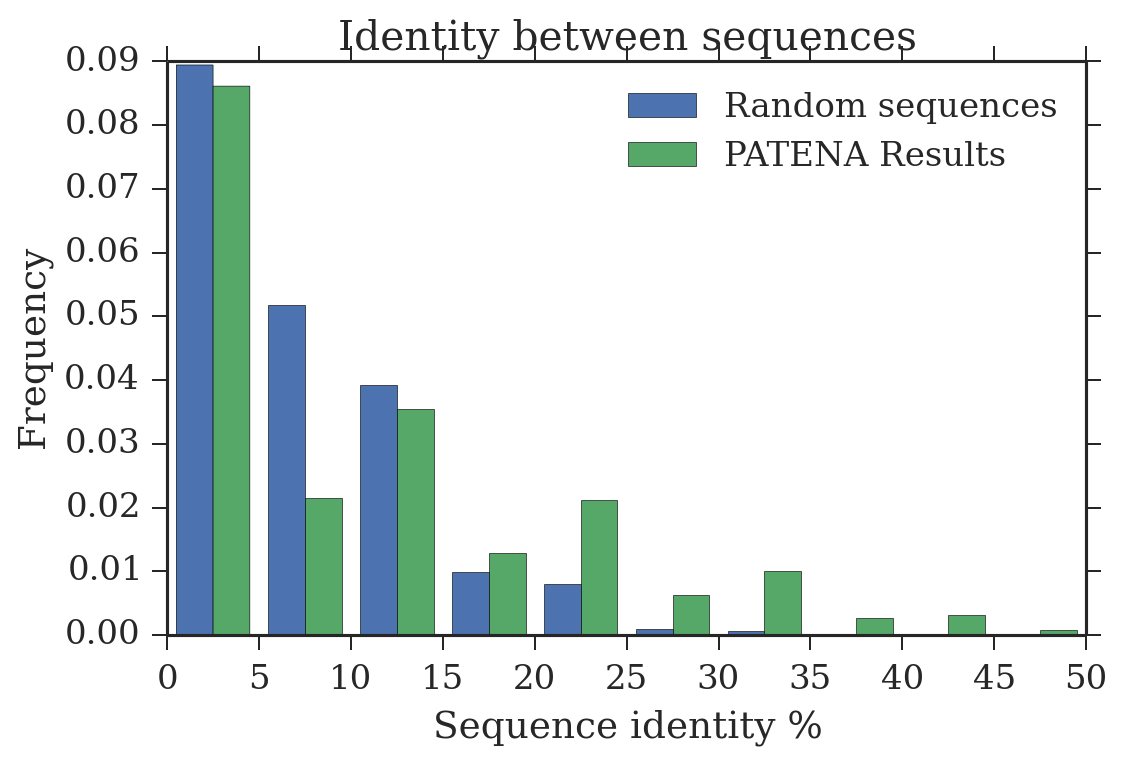
\includegraphics[width=240px,height=185px]{img/resultados/againstAll-random.png}
    \label{fig:identity-b}
%     \caption{Identidad entre cada par posible de secuencias resultantes(74*74)}
  \end{subfigure}
  \caption{Histograma de identidad entre las secuencias resultantes entre si(derecha) y entre estas y la secuencia inicial(izquierda)}
  \label{fig:identity}
\end{figure}



Los diseños resultantes obtenidos a partir de una misma secuencia inicial no poseen similitud entre sí, lo cual puede entenderse como el resultado de las propiedades estocásticas del método que generan 
una gran divergencia entre distintas ejecuciones independientes.
Por otro lado, las secuencias resultantes ciertamente muestran una similitud remanente con la secuencia inicial, lo cual podría indicar que, en cada ejecución, las mutaciones no se distribuyen de manera uniforme entre las posiciones.

Sin embargo, este análisis de identidad global entre secuencias no permite conocer si la similitud se encuentra localizada en alguna posición especifica.
La extracción de un logo secuencial a partir del conjunto de resultados permite analizar ,en detalle(para cada posición), la similitud entre los resultados. 
Un logo secuencial muestra en una representación gráfica de la similitud en un conjunto de secuencias\cite{schneider1990sequence}, 
en este caso entre los resultados de las 74 corridas independientes(figura \ref{fig:logo}).
% generar una respresentación gráfica más relevante de la similitud entre estos.
% Una mejor representación de esta similitud entre las secuencias resultantes se obtiene extrayendo un logo secuencial a partir de este conjunto de resultados.

\begin{figure}[h]
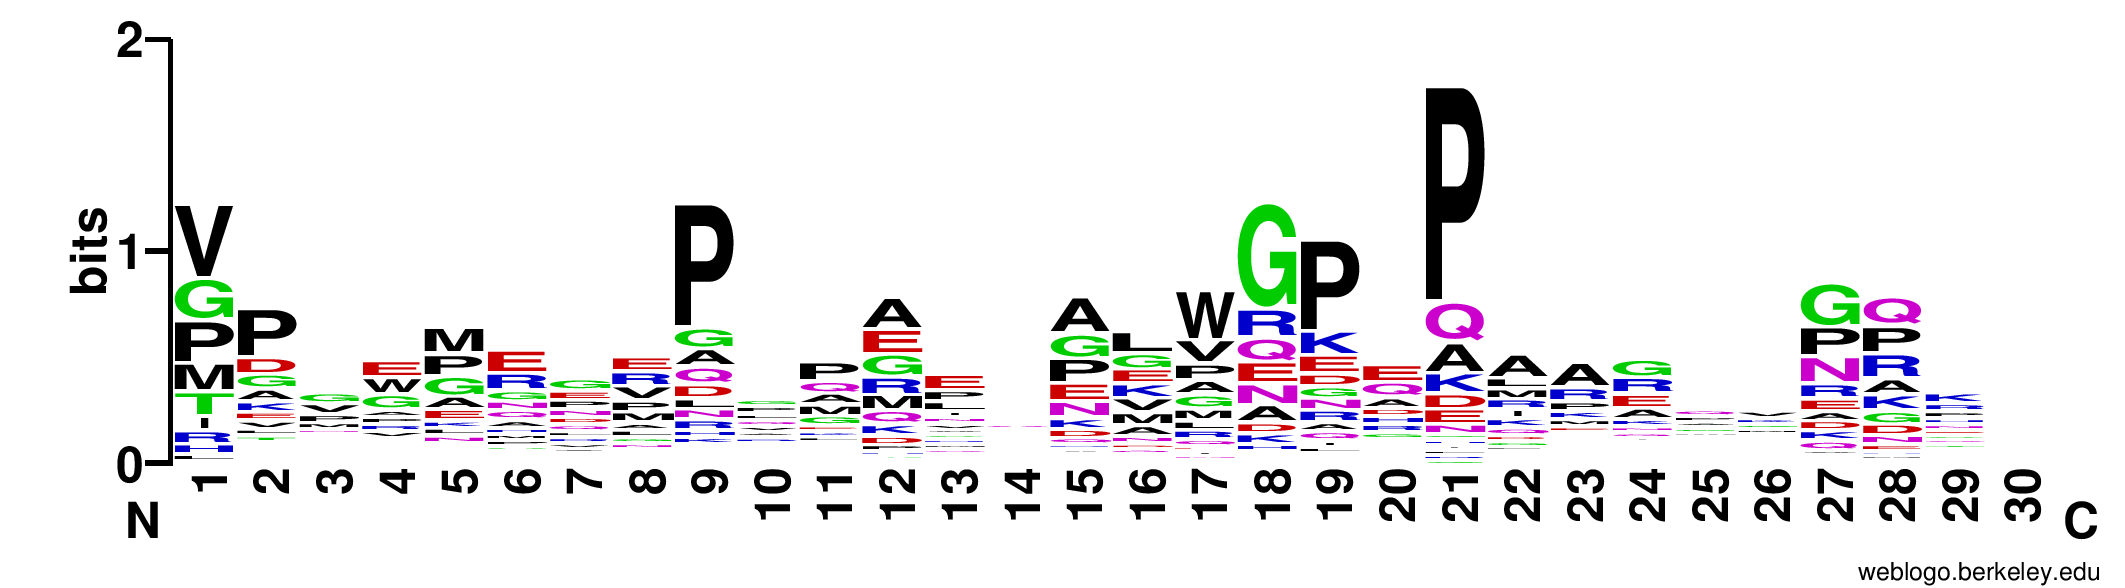
\includegraphics[width=\textwidth]{img/resultados/logo.png}
\caption{Representación gráfica de la similitud secuencial. Obtenida de \cite{crooks2004weblogo}}
\label{fig:logo}
\end{figure}

Como se ve, la similitud entre los resultados se concentra en las posiciones que inicialmente  
% los residuos que mas se repiten entre las secuencias resultantes son los correspondientes a las posiciones que inicialmente
poseían residuos de Glicina y Prolina (posiciones 9,18,19,21), y los residuos mas representados en estas posiciones son, justamente, los mismos que se encontraban en la secuencia inicialmente. 
Si revisamos los resultados del análisis de mutaciones para cada posición(figura \ref{fig:mutationPerSite}), veremos que, si bien no hay una diferencia significativa, 
son justamente estas posiciones las que tienen menores porcentajes medio de mutación.
Por otro lado, el resto de las posiciones mantienen una gran diversidad en cuanto a aminoácidos, cómo se ve en la figura \ref{fig:logo},
por lo tanto, la similitud en estas posiciones parece ser producto de la falta de mutaciones.
Al parecer, estas mantienen un valor de puntaje bajo a lo largo de la ejecución y pueden, en algunos casos, finalizar la ejecución sin sufrir ninguna mutación, manteniendo los residuos iniciales intactos en el diseño final.
% y por lo tanto que los residuos iniciales se mantienen intactos.
% Sin embargo, no hay una diferencia significativa en el porcentaje de mutaciones promedio que se aplican en estas posiciones, por lo que es posible que esta similitud puntual se deba que la
% La menor cantidad de mutaciones en estas posiciones se ve reflejada en la similitud secuencial entre los diseños resultantes.





